\documentclass{article}
\usepackage{amsmath,amssymb,amsfonts}
\usepackage{latexsym}
\usepackage{graphicx}
\usepackage{verbatim}
\usepackage{booktabs}
\usepackage[usenames,dvipsnames,svgnames,table]{xcolor}
\usepackage{todonotes} % Required for the boxes that questions appear in

\newcommand{\mybox}[1]
{
\par\noindent
\todo[inline, backgroundcolor=SkyBlue!40,bordercolor=SkyBlue,size=\large]{\textbf{#1}}
\vspace{1em}
}

\usepackage[top=25mm, bottom=25.4mm, left=16.7mm, right=18.9mm]{geometry}

\usepackage{fancyhdr}
\pagestyle{fancy}
\lhead{Numerical Analysis Assignment \#5 }
\chead{Xinglu Wang \quad 3140102282}
%\renewcommand{\headrulewidth}{0.3pt}

\usepackage[framed,numbered,autolinebreaks,useliterate,final]{mcode}
\usepackage{listings}
\title{\textbf{Numerical Analysis Assignment \#5}}
\author{Xinglu Wang \qquad Student Number: 3140102282
    \\ %\vspace{0.5em}
    College of Information Science \& Electronic Engineering}
\date{}

\makeatletter
\def\@seccntformat#1{%
  \expandafter\ifx\csname c@#1\endcsname\c@section\else
  \csname the#1\endcsname\quad
  \fi}
\makeatother

\usepackage{multirow}

\usepackage{sectsty}
\sectionfont{\color{NavyBlue}\selectfont}
\subsectionfont{\color{SkyBlue}\itshape\selectfont}

\newcommand{\abs}[1]{\left| #1 \right| }
\newcommand{\norm}[1]{\left\| {#1} \right\|}

\begin{document}
\maketitle
\section{problem 1}
\begin{figure}
  \centering
  % Requires \usepackage{graphicx}
  \includegraphics[width]{../xxx.png}\\
  \caption{}\label{}
\end{figure}

\begin{description}
\item[a).]
For this problem, if we use formula derived on the book, which means using $f=p1x+p2$ to fit. We get the coefficients (with 95\% confidence bounds):
 \[      p1 =      0.7525  (0.2317, 1.273) \text{  and  }
       p2 =      -3.199  (-8.307, 1.909)\]
Here, $E=\frac{-p2}{p1}=4.25\neq5.3$ then the true value will be unused. So we must regard that $E$ is known.
\[\begin{array}{l}
E({a_0},{a_1}) = {E_2}({a_0},k{a_0})
 = \sum\limits_{i = 1}^m {{{\left[ {{y_i} - (k{a_0}{x_i} + {a_0})} \right]}^2}}
\end{array}\]where k is constant $-\frac{1}{E}$, then
\[\begin{array}{l}
\frac{dE}{d{a_0}} = 0\\
 \Rightarrow {a_0} =  - 4.59\\
 \Rightarrow {a_1} =  - \frac{1}{{5.3}}{a_0} = 0.8996
\end{array}\]
And the error should be mean error:  $\frac{1}{3}\sum\limits_{i = 1}^m {{\left[ {{y_i} - (k{a_0}{x_i} + {a_0})} \right]}^2}=0.136$ \\
Meanwhile, we can use linear fittype in matlab to fit $a_1$.
\lstinputlisting{../mcode/LeastSquare.m}
\item[b).]
Similarly, $a1=0.9052$ and $E(a1)= \frac{1}{7}\sum\limits_{i = 1}^m {{\left[ {{y_i} - (k{a_0}{x_i} + {a_0})} \right]}^2}=0.128$. So $a_1=0.9052$ is more accurate with more data points.
\end{description}
\section{problem 2}
On the one hand, we can use the formula
\begin{center}
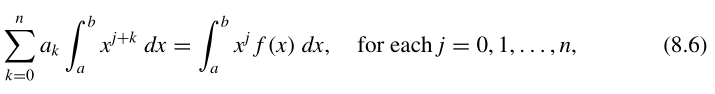
\includegraphics[width=8cm]{../pic/p2_1.png}
\end{center}
But the complexity of calculating an linear system will be great. So we choose The set of Legendre polynomials ${P_n (x)}$, which is orthogonal on $[-1,1]$
with respect to the weight function $w(x) \equiv 1$.
\[\begin{array}{l}
{P_0}(x) = 1\\
{P_1}(x) = x\\
{P_2}{x} = x^2-\frac{1}{3}
\end{array}\]

\begin{description}
  \item[a).]
  My answer is
  \[f(x)=\frac{10}{3}-2x\]
  I find that the linear least sqaure polynominal approximation is just discard the item with high power, because we can see the accurate form with respect to Legendre polynomials is $f(x)=\frac{10}{3}-2x+(x^2-\frac{1}{3})$, and to approximate is to discard $(x^2-\frac{1}{3})$.
  \item[b).]
  Similarly, my answer is \[ f(x)=0.6x \]
\end{description}

\section{problem 3}
According to Gram-Schmidt Process,
\begin{center}
  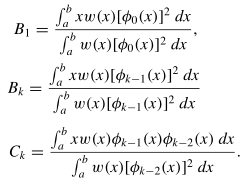
\includegraphics[width=4.5cm]{../pic/p3_2.png}
\end{center}
These are the first few Laguerre polynomials:
\[\begin{array}{l}
{\phi_0}(x) = 1\\
{\phi_1}(x) =   x - 1\\
{\phi_2}(x) = {x^2} - 4x + 2\\
{\phi_3}(x) =   {x^3} - 9{x^2} + 18x - 6

\end{array}\]

\section{problem 4}
Using the Three-point Startpoint formula for $x_1$ , Three-point Midpoint formula for $x_2, x_3$ and Endpoint for $x_4$. We get
\begin{description}
\item[a).]
\begin{center}
\begin{tabular}{ll}
\hline
x&f'(x)\\\hline
1.1&17.76\\
1.2&22.19\\
1.3&27.1\\
1.4&32.51\\
\hline
\end{tabular}
\end{center}
\item[b).]
\begin{center}
\begin{tabular}{ll}
\hline
{\small x}&{\small f'(x)}\\
\hline
{\small 8.1}&{\small 3.09}\\
{\small 8.3}&{\small 3.12}\\
{\small 8.5}&{\small 3.14}\\
{\small 8.7}&{\small 3.16}\\
\hline
\end{tabular}
\end{center}
\end{description}
\section{problem 5}
We need to complete the table below,
\begin{center}
\begin{tabular}{ccccc} \hline
$O(h^2)$ & $O(h^4)$ &$O(h^6)$ \\
\hline
$N_0(h)$         		  &    								   & 										\\
$N_0(\frac{h}{3})$  & $N_1(h)$    				 &  									\\
$N_0(\frac{h}{3^2})$	& $N_1(\frac{h}{3})$   & $N_2(h)$  					\\
 \hline
\end{tabular}
\end{center}
\begin{center}
Table 5.1 Iteration of a Richardson's Extrapolation Method
\end{center}
First, to calculate $N_1$, we know
\begin{equation}
\begin{array}{c}
M = {N_0}(h) + K{h^2} + O({h^4})\;\\
M = N(\frac{h}{3}) + K\frac{{{h^2}}}{9} + O({h^4})
\end{array}
\end{equation}
We get
\[\begin{array}{l}
M = \frac{1}{8}\left[ {9N(\frac{h}{3}) - N(h)} \right] + O({h^4})\\
 \buildrel\textstyle.\over= {N_1}(h) + O({h^4})
\end{array}\]
Substitute $h$ with $\frac{h}{3}$, we get $N_1(\frac{h}{3})=\frac{1}{8}\left[ {9N(\frac{h}{9}) - N(\frac{h}{3})} \right]$
\\Then iterate again, we get
$N_2(h)=\frac{1}{{640}}{N_0}(h) - \frac{9}{{64}}{N_0}(\frac{h}{3}) + \frac{{729}}{{640}}{N_0}(\frac{h}{9})$. So finally,

\[M = \frac{1}{{640}}{N_0}(h) - \frac{9}{{64}}{N_0}(\frac{h}{3}) + \frac{{729}}{{640}}{N_0}(\frac{h}{9}) + O({h^6})\]


\section{Problem 6}
My answer is:
\begin{center}\begin{tabular}{l|ll}
\hline
 & Trapezoidal & Simpson \\
\hline
$\int_{-0.25}^{0.25}{cos^2x}$ &{0.469395640472593} & 0.489798546824198\\
$\int_{0}^{0.5}{xln(x+1)}$&{0.086643397569993}&0.052854638560979\\
$\int_0.75^1.3{sin^2x-2xsinx+1}$&{-0.037024252723997 }&-0.020271589910295\\
$\int_e^{e+1} {\frac{1}{{x\ln x}}dx} $&{0.286334172478335 }&0.272670452444963\\
\hline
\end{tabular}
\end{center}
The code to implement methods is shown below:
\lstinputlisting{../mcode/Trape.m}
\lstinputlisting{../mcode/Simps.m}
\section{Problem 7}
Using $h_{n}={\tfrac {1}{2^{n}}}(b-a)$, Romberg method can be inductively defined by
\[\begin{array}{l}
R(0,0) = {h_1}(f(a) + f(b))\\
R(n,0) = {\textstyle{1 \over 2}}R(n - 1,0) + {h_n}\sum\limits_{k = 1}^{{2^{n - 1}}} f (a + (2k - 1){h_n})\\
R(n,m) = R(n,m - 1) + {\textstyle{1 \over {{4^m} - 1}}}(R(n,m - 1) - R(n - 1,m - 1))\\
\end{array}\]
where $n\geq m\, $ and $ m\geq 1\,$.
Just consider $n=m=3$, my answer is
\begin{center}\begin{tabular}{ll}
\hline
$\int_{-1}^{1}{cos^2x}$&{ 1.452814}\\
$\int_{-0.75}^{0.75}{xln(x+1)}$&{ 0.327959}\\
$\int_1^4{sin^2x-2xsinx+1}$&{ 1.387063}\\
$\int_e^{2e} {\frac{1}{{x\ln x}}dx} $&{ 0.526816}\\
\hline
\end{tabular}
\end{center}
\lstinputlisting{../mcode/Romb.m}
\section{Problem 8}
\textbf{a).}
We can compare Euler's method with analytic solution, since this ODE have analytic solution $\frac{t}{\mathrm{log}\!\left(t\right) + 1}$:
\begin{center}\begin{tabular}{lll}
\hline
T &Euler's method & $\frac{t}{\mathrm{log}\!\left(t\right) + 1}$\\\hline
1&1&1\\
\hline
1.1&1.004281728&1\\
\hline
1.2&1.014952314&1.008264463\\
\hline
1.3&1.029813689&1.021689472\\
\hline
1.4&1.047533919&1.038514734\\
\hline
1.5&1.067262354&1.057668192\\
\hline
1.6&1.088432687&1.078461094\\
\hline
1.7&1.110655052&1.100432165\\
\hline
1.8&1.133653556&1.123262052\\
\hline
1.9&1.157228433&1.146723597\\
\hline
2&1.181232218&1.17065157\\
\hline
\end{tabular}\end{center}
\begin{center}
  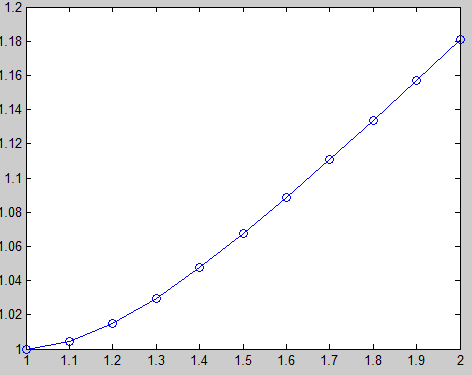
\includegraphics[width=7.5cm]{../pic/p8_2.png}\\
\end{center}

Apparently, Euler's method is not very accurate. On the one hand h is a kind of large, and on the other hand the LTE is $O(h)$ itself.
\lstinputlisting{../mcode/myode.m}
\textbf{b).}
Similarly, my answer is
\begin{center}\begin{tabular}{ll}
\hline
T&Y\\
\hline
1&0\\
\hline
1.2&0.2\\
\hline
1.4&0.438888889\\
\hline
1.6&0.721242756\\
\hline
1.8&1.052038032\\
\hline
2&1.437251148\\
\hline
2.2&1.884260805\\
\hline
2.4&2.402269589\\
\hline
2.6&3.002837165\\
\hline
2.8&3.700600705\\
\hline
3&4.514277428\\
\hline
\end{tabular}
\end{center}
\begin{center}
  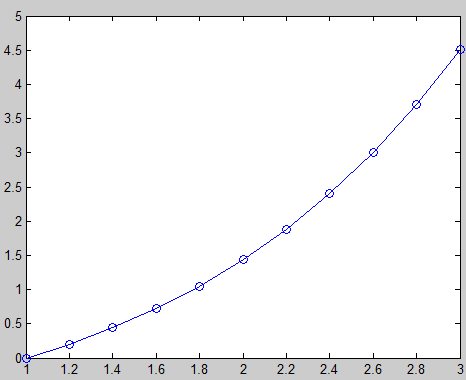
\includegraphics[width=7.5cm]{../pic/p8_3.png}\\
\end{center}

\end{document}
